\documentclass{standalone}
\usepackage{tikz}
\usepackage{standalone}
\usetikzlibrary{calc}

\begin{document}
    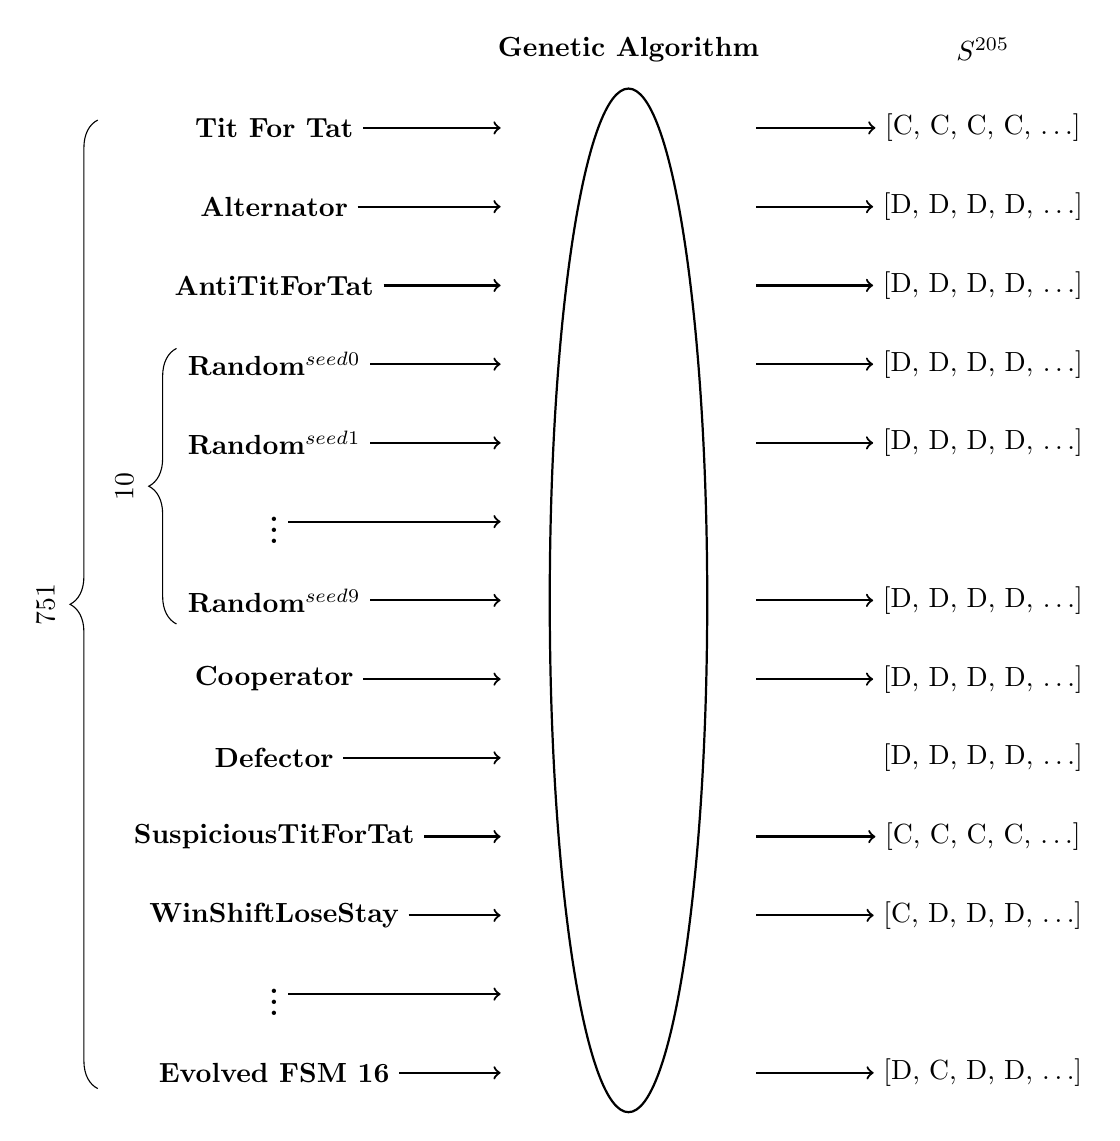
\begin{tikzpicture}
    \node[font=\bfseries] (0) at (0, 0) {Tit For Tat};
    \node[font=\bfseries] (1) at ($(0)+(0, -1)$) {Alternator};
    \node[font=\bfseries] (2) at ($(1)+(0, -1)$) {AntiTitForTat};
    \node[font=\bfseries] (3) at ($(2)+(0, -1)$) {Random$^{\text{seed} 0}$};
    \node[font=\bfseries] (4) at ($(3)+(0, -1)$) {Random$^{\text{seed} 1}$};
    \node[font=\bfseries] (5) at ($(4)+(0, -1)$) {$\vdots$};
    \node[font=\bfseries] (6) at ($(5)+(0, -1)$) {Random$^{\text{seed} 9}$};
    \node[font=\bfseries] (7) at ($(6)+(0, -1)$) {Cooperator};
    \node[font=\bfseries] (8) at ($(7)+(0, -1)$) {Defector};
    \node[font=\bfseries] (9) at ($(8)+(0, -1)$) {SuspiciousTitForTat};
    \node[font=\bfseries] (10) at ($(9)+(0, -1)$) {WinShiftLoseStay};
    \node[font=\bfseries] (11) at ($(10)+(0, -1)$) {$\vdots$};
    \node[font=\bfseries] (12) at ($(11)+(0, -1)$) {Evolved FSM 16};

    \draw [decorate,decoration={brace,amplitude=10pt, mirror,raise=4pt},yshift=0pt] (-1.1, -2.8) -- (-1.1, -6.3) node [rotate=90, midway, yshift=0.8cm] {10};
    \draw [decorate,decoration={brace,amplitude=10pt, mirror,raise=4pt},yshift=0pt] (-2.1, 0.1) -- (-2.1, -12.2) node [rotate=90, midway, yshift=0.8cm] {751};

    \node (dummy0) at (3, 0) {};
    \node (dummy1) at ($(dummy0)+(0, -1)$) {};
    \node (dummy2) at ($(dummy1)+(0, -1)$) {};
    \node (dummy3) at ($(dummy2)+(0, -1)$) {};
    \node (dummy4) at ($(dummy3)+(0, -1)$) {};
    \node (dummy5) at ($(dummy4)+(0, -1)$) {};
    \node (dummy6) at ($(dummy5)+(0, -1)$) {};
    \node (dummy7) at ($(dummy6)+(0, -1)$) {};
    \node (dummy8) at ($(dummy7)+(0, -1)$) {};
    \node (dummy9) at ($(dummy8)+(0, -1)$) {};
    \node (dummy10) at ($(dummy9)+(0, -1)$) {};
    \node (dummy11) at ($(dummy10)+(0, -1)$) {};
    \node (dummy12) at ($(dummy11)+(0, -1)$) {};
    
    \node[font=\bfseries] (h) at (4.5, 1) {Genetic Algorithm};
    \draw [thick] (4.5, -6) ellipse (1cm and 6.5cm);

    \draw (0) edge[->, out=0, in=180, thick] (dummy0);
    \draw (1) edge[->, out=0, in=180, thick] (dummy1);
    \draw (2) edge[->, out=0, in=180, thick] (dummy2);
    \draw (3) edge[->, out=0, in=180, thick] (dummy3);
    \draw (4) edge[->, out=0, in=180, thick] (dummy4);
    \draw (5) edge[->, out=0, in=180, thick] (dummy5);
    \draw (6) edge[->, out=0, in=180, thick] (dummy6);
    \draw (7) edge[->, out=0, in=180, thick] (dummy7);
    \draw (8) edge[->, out=0, in=180, thick] (dummy8);
    \draw (9) edge[->, out=0, in=180, thick] (dummy9);
    \draw (10) edge[->, out=0, in=180, thick] (dummy10);
    \draw (11) edge[->, out=0, in=180, thick] (dummy11);
    \draw (12) edge[->, out=0, in=180, thick] (dummy12);

    \node (dummy_1_0) at (6, 0) {};
    \node (dummy_1_1) at ($(dummy_1_0)+(0, -1)$) {};
    \node (dummy_1_2) at ($(dummy_1_1)+(0, -1)$) {};
    \node (dummy_1_3) at ($(dummy_1_2)+(0, -1)$) {};
    \node (dummy_1_4) at ($(dummy_1_3)+(0, -1)$) {};
    \node (dummy_1_5) at ($(dummy_1_4)+(0, -1)$) {};
    \node (dummy_1_6) at ($(dummy_1_5)+(0, -1)$) {};
    \node (dummy_1_7) at ($(dummy_1_6)+(0, -1)$) {};
    \node (dummy_1_8) at ($(dummy_1_7)+(0, -1)$) {};
    \node (dummy_1_9) at ($(dummy_1_8)+(0, -1)$) {};
    \node (dummy_1_10) at ($(dummy_1_9)+(0, -1)$) {};
    \node (dummy_1_11) at ($(dummy_1_10)+(0, -1)$) {};
    \node (dummy_1_12) at ($(dummy_1_11)+(0, -1)$) {};

    \node[font=\bfseries] (h) at (9, 1) {$S^{205}$};
    \node (bf0) at (9, 0)  {[C, C, C, C, $\dots$]};
    \node (bf1) at ($(bf0)+(0, -1)$) {[D, D, D, D, $\dots$]};
    \node (bf2) at ($(bf1)+(0, -1)$) {[D, D, D, D, $\dots$]};
    \node (bf3) at ($(bf2)+(0, -1)$) {[D, D, D, D, $\dots$]};
    \node (bf4) at ($(bf3)+(0, -1)$) {[D, D, D, D, $\dots$]};
    \node (bf5) at ($(bf4)+(0, -1)$) {};
    \node (bf6) at ($(bf5)+(0, -1)$) {[D, D, D, D, $\dots$]};
    \node (bf7) at ($(bf6)+(0, -1)$) {[D, D, D, D, $\dots$]};
    \node (bf8) at ($(bf7)+(0, -1)$) {[D, D, D, D, $\dots$]};
    \node (bf9) at ($(bf8)+(0, -1)$) {[C, C, C, C, $\dots$]};
    \node (bf10) at ($(bf9)+(0, -1)$) {[C, D, D, D, $\dots$]};
    \node (bf11) at ($(bf10)+(0, -1)$) {};
    \node (bf12) at ($(bf11)+(0, -1)$) {[D, C, D, D, $\dots$]};

    \draw (dummy_1_0) edge[->, out=0, in=180, thick] (bf0) {};
    \draw (dummy_1_1) edge[->, out=0, in=180, thick] (bf1) {};
    \draw (dummy_1_2) edge[->, out=0, in=180, thick] (bf2) {};
    \draw (dummy_1_3) edge[->, out=0, in=180, thick] (bf3) {};
    \draw (dummy_1_4) edge[->, out=0, in=180, thick] (bf4) {};
    \draw (dummy_1_6) edge[->, out=0, in=180, thick] (bf6) {};
    \draw (dummy_1_7) edge[->, out=0, in=180, thick] (bf7) {};
    \draw (dummy_1_9) edge[->, out=0, in=180, thick] (bf9) {};
    \draw (dummy_1_10) edge[->, out=0, in=180, thick] (bf10) {};
    \draw (dummy_1_12) edge[->, out=0, in=180, thick] (bf12) {};
    \end{tikzpicture}
\end{document}